\chapter{Integration in a Real Project} \label{ch:integration}

To demonstrate the real utility and effectiveness of the previously created decentralized identity management \gls{ssi} framework, it was integrated as an authentication process 
into an ongoing project at Links Foundation, known as \textit{Data Cellar}. Later, in addition to the integration of this system, the entire \gls{gui} of the application was also developed.

In this chapter, we will first deal with what \textit{Data Cellar} is and what the initial state of the project was. Then, we will examine in detail the entire integration process 
and the final graphical result of the application.

\section{Overview of Data Cellar}

\textit{Data Cellar} is an energy data center, geographically located within the European Union, whose main activities consist of the construction of a federated energy data space in 
order to enable the creation, growth, and support of local energy communities \cite{datacellarproject}. That initiative is based on an innovative rewarded private metering approach,, stressing 
successful integration, simplicity of the interactions, guaranteeing integration with other energy data spaces in the \gls{eu} and providing the actors with the services and tools
they need for their own actions.

As part of this four-year project, Links Foundation endeavors to decentralize various functionalities of the data center, resulting in enhanced security, speed, 
distribution, and additional benefits inherent to blockchain and decentralized architectures.

Naturally, being a project in development within the company and at the outset of this process, in its initial version, the set of functionalities offered by this 
decentralized version is still limited compared to its standard operational version at the European level.

\section{Initial Project Status}

In its decentralized application form, the \textit{Data Cellar} project comprised a set of smart contracts enabling various functionalities (briefly discussed later), invoked through
a backend written in \textit{NestJs}, with its interface generated via \textit{Swagger}. \textit{Swagger}, which is an \gls{api} documentation tool, streamlines the documentation of RESTful \gls{api}s, so that 
the developers could focus on the code while not bothering about the manual creation of documentation.

\subsection{Development Environment}

The execution environment of the project was simulated using \textit{Docker}. \textit{Docker} is an open-source platform that is used for application creation, distribution, and execution, 
all within containers. \textit{Docker} containers represent a modern form of virtualization that allows developers to bundle applications and all their dependencies (such as 
libraries, frameworks, and other components) into a self contained unit known as a "container" \cite{docker}.

Specifically, in this case, three containers were executed: 

\begin{itemize}
  \item \textbf{Ganache:} An Ethereum-based private blockchain simulation containing pre-created accounts with visible private keys and a fund of 100 ETH.
  \item \textbf{Postgres:} The off-chain database for storing user information.
  \item \textbf{Redis:} The service for initializing and using queues to handle requests on the blockchain.
\end{itemize}

As can be seen from these containers, the user identity management system was still completely centralized, using a database implemented through \textit{Prisma}, in which user IDs, 
accounts and private keys were stored.

\subsection{Offered Functionalities} 

The key aspect of the initial version of the project was the digitization of energy data and its exchange among users through the purchase of one-time and periodic licenses.
Features offered included:

\begin{itemize}
  \item User registration, which includes the assignment of an address to the new user enabling them to buy and sell digital assets on the blockchain. 
  \item Visualization of datasets and associated licenses. 
  \item Upload of datasets and associated licenses. 
  \item Purchase of licenses associated with datasets.
  \item Deletion of licenses associated with datasets and the datasets themselves.
  \item Visualization of DataCellar Token balance.
\end{itemize}

\section{Integration Process}

Following the guidelines provided, from the initial version, of the \textit{Data Cellar} project, in the form of a decentralized application, the decision was made to continue using 
\textit{Ganache} as a local network, running through a \textit{Docker} container, rather than using Ethereum testnets, such as \textit{Goerli} and \textit{Sepolia}, as was done for the creation of the 
standalone framework for managing \gls{ssi}.

First, the previously created framework was adapted to work with \textit{Ganache}, and the configuration of MetaMask was then modified. In fact, among other functions, MetaMask 
allowed the addition of new local networks, such as \textit{Ganache}, and the import of corresponding accounts into the wallet. As a final step regarding the blockchain aspect, 
the existing script, which loaded all the contracts used to execute the project's functionalities upon \textit{Docker} startup, had the \gls{ssi} framework smart contract acting as a 
registry and the one used by \textit{ethr-did} for \gls{did} management added.

Subsequently, the code was modified, changing its structure almost completely. This was done because all the \gls{api}s, which invoked the functions, defined within the smart 
contract, had to be moved from the backend, where it was executed only because the users' private keys were stored in plain text in the database, to the frontend, to be 
executed using MetaMask, which allows transactions to be signed without exposing the users' private keys.

During this code change, the use of the database, thus \textit{Prisma} and \textit{Postgres}, the use of queues, as they are not supported by MetaMask, and the use of \textit{Swagger} were completely 
eliminated, as a new \gls{gui} was created.

\section{Final Application}

The second version of the \textit{Data Cellar} corresponds to the final application that has been built, in the form of a decentralized application that has been integrated with the 
SSI framework and is further enriched with a dynamic and user-friendly frontend.

The functionalities of the second version of the \textit{Data Cellar} can be divided into functionalities that relate to the \gls{ssi} framework, those designed for visitors, and those 
for registered members.These functionalities include:

\begin{itemize}
  \item \textbf{SSI functionalities:}
  \begin{itemize}
      \item Connection to \textit{Data Cellar} (access as a visitor)
      \item Registration to \textit{Data Cellar} (sign up as a member)
      \item Authentication in \textit{Data Cellar} (sign in as a member)
      \item Delete your \textit{Data Cellar} account
  \end{itemize}
  
  \item \textbf{Visitor functionalities:}
  \begin{itemize}
      \item View all datasets available in \textit{Data Cellar}
      \item View all available licenses for each dataset
  \end{itemize}
  
  \item \textbf{Member functionalities:}
  \begin{itemize}
      \item View the balance of ETH and DataCellar tokens
      \item Convert ETH to DataCellar tokens
      \item Add new datasets in \textit{Data Cellar}
      \item Create new licenses, single-use, or periodic, for your datasets
      \item View, edit, and delete your own datasets
      \item View, edit, and delete your own licenses
      \item Buy licenses for datasets added by other users
      \item View purchased licenses and reference datasets
      \item Consume purchased licenses
  \end{itemize}
\end{itemize}

\subsection{Backend Implementation}

To follow the guidelines, provided by the first version of this project, the backend remained written in \textit{NestJs}, using the structure proposed by the language, consisting of 
Module, Controller and Service files. On the logical level, however, within the backend, which acts as a server, only the two features present in the framework for \gls{ssi} 
management remained, namely:

\begin{itemize}
  \item Verification of the user's signature and generation of an access token (which will be placed in the session cookie to verify user authentication)
  \item Generation of a \gls{vc} demonstrating the sign-up to DataCellar (the user must provide it in order to access the dApp)
\end{itemize}

\subsection{Frontend Development}

As in the previous case, the frontend, realized using \textit{React}, covers the most substantial part of the application. It contains not only the entire graphical interface but 
also the authentication process of the \gls{ssi} framework, explained earlier, enriched by the de-registration functionality, along with all the \gls{api}s invoking the functionalities 
defined in the smart contracts of the \textit{Data Cellar} project.

The \gls{gui}, in order to be user-friendly, has been enriched with confirmation modals for the most important operations, which the user can perform, and automatically 
disappearing error and success alerts, which cover all possible outcomes, of the various features the user can perform, within the application.

Finally, let us then briefly examine the two main pages that make up the \textit{Data Cellar} project in its second version in the form of a browser \gls{dapp}. 

\subsubsection{Home Page}

\begin{figure}[h]  
  \centering
  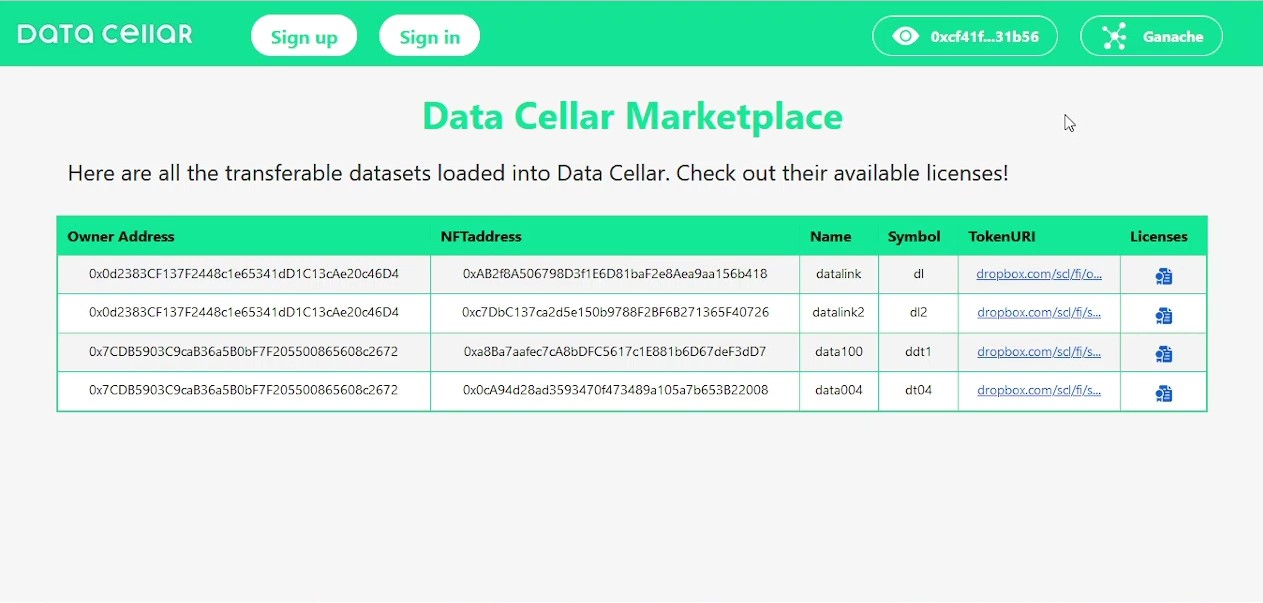
\includegraphics[width=1\textwidth]{Images/c6_4.jpg} 
  \caption{The marketplace in the Data Cellar Home page.}
\end{figure}

The initial page shows the \textit{Data Cellar} marketplace, where all transferable datasets created by other users are visible. Various information is provided for each dataset, 
from the address of the owner, to the \gls{uri} of the Token, which actually contains the energy data.

Clicking on the license symbol takes you to the corresponding page, which shows for the referenced dataset all available licenses, indicating for each of them various 
information, including the price in DataCellar Token, i.e., the currency used within the application. 

\begin{figure}[h]  
  \centering
  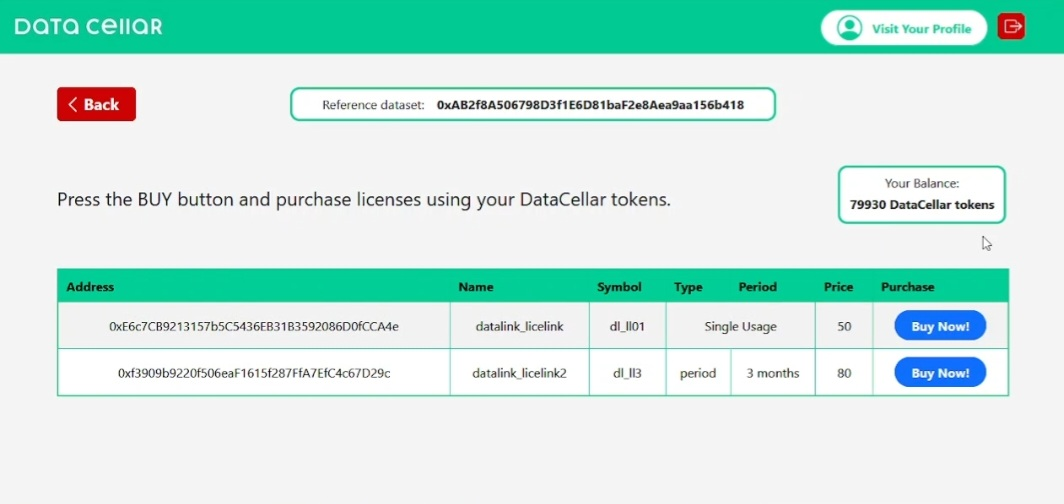
\includegraphics[width=1\textwidth]{Images/c6_5.jpg} 
  \caption{List of licenses for a specific dataset, after authentication process.}
\end{figure}

Authenticated members can purchase these licenses, either for a period or for single use, in the latter case, a modal allowing the definition of the quantity of licenses to
purchase together is provided.

\subsubsection{Profile Page}

By clicking on the "visit your profile" button in the navigation bar, users can access their profile. Within it are various sections covering all the personal functionality 
executable by the user:

\newpage

\begin{itemize}
  \item \textbf{General Information:} Contains the user's information obtained from the token placed in the session cookie.
  
  \begin{figure}[h]  
    \centering
    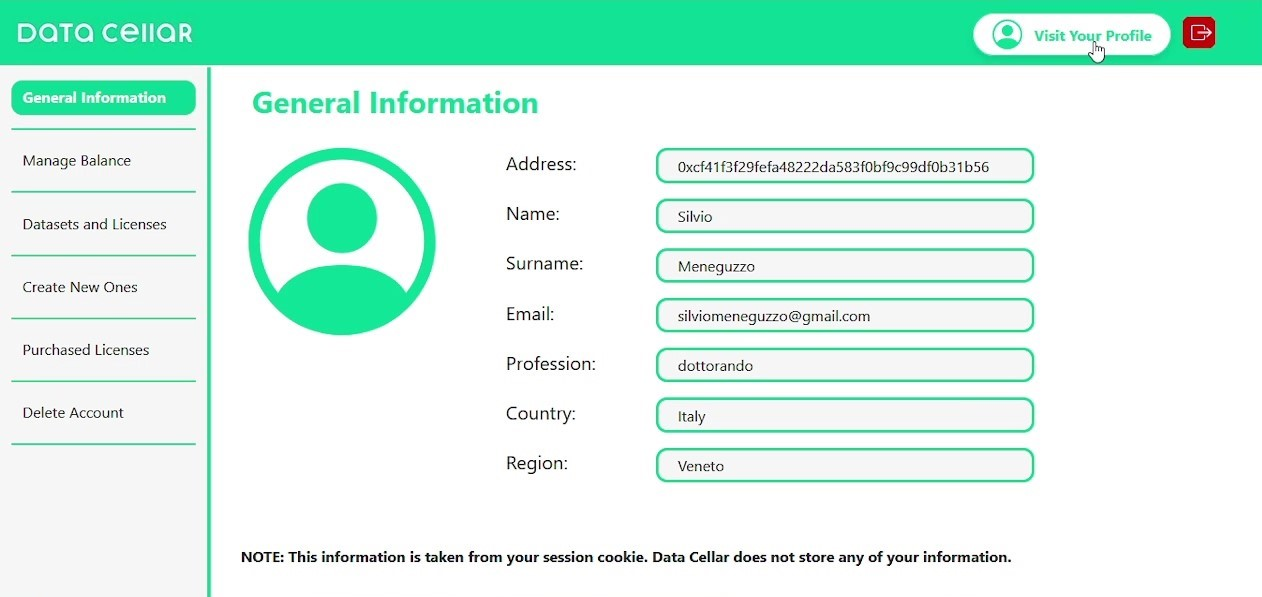
\includegraphics[width=0.8\textwidth]{Images/c6_6.jpg} 
    \caption{Page to view user's personal information.}
  \end{figure}
  
  \item \textbf{Manage Balance:} Displays the user's DataCellar Token and Ethereum balance, also allowing conversion of new ETH to DataCellar tokens.
  
  \begin{figure}[h]  
    \centering
    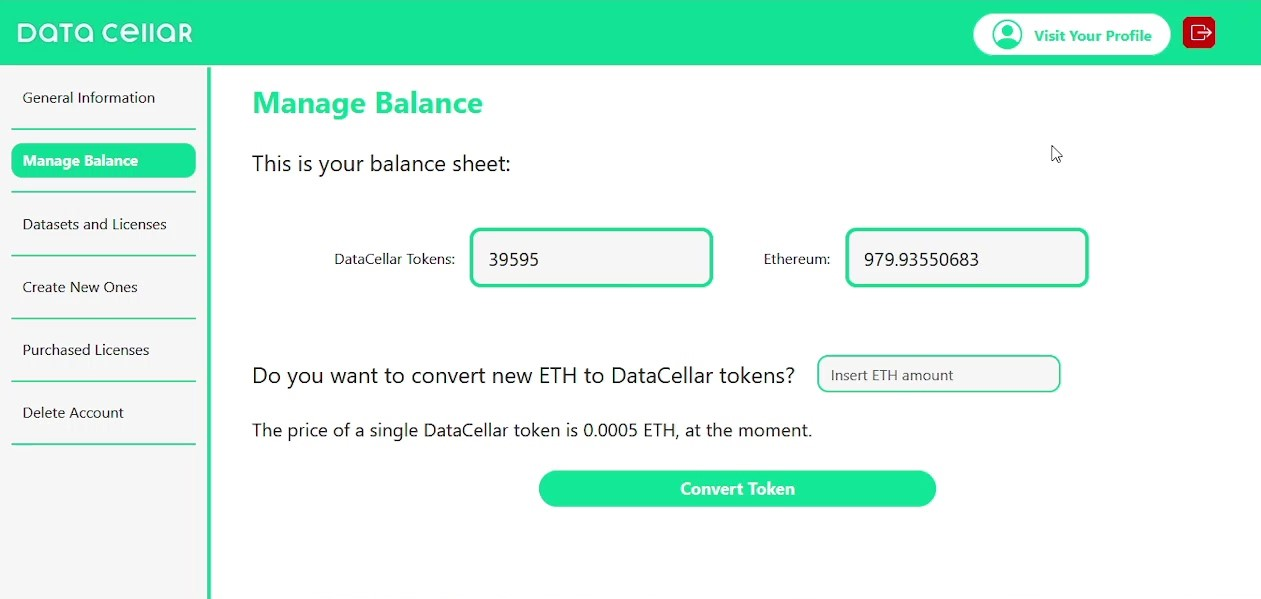
\includegraphics[width=0.8\textwidth]{Images/c6_7.jpg} 
    \caption{Page to manage user's DataCellar tokens.}
  \end{figure}
  
  \item \textbf{Datasets and Licenses:} Displays all datasets created by the user; each can be edited or deleted, using the corresponding buttons that open the relevant 
  modals. Also, by clicking on the license symbols, the user can view all the licenses he has created for that dataset. By accessing the dedicated page, the user can also 
  edit and delete each license through the corresponding buttons and modals, as in the previous case. 
  
  \begin{figure}[h]  
    \centering
    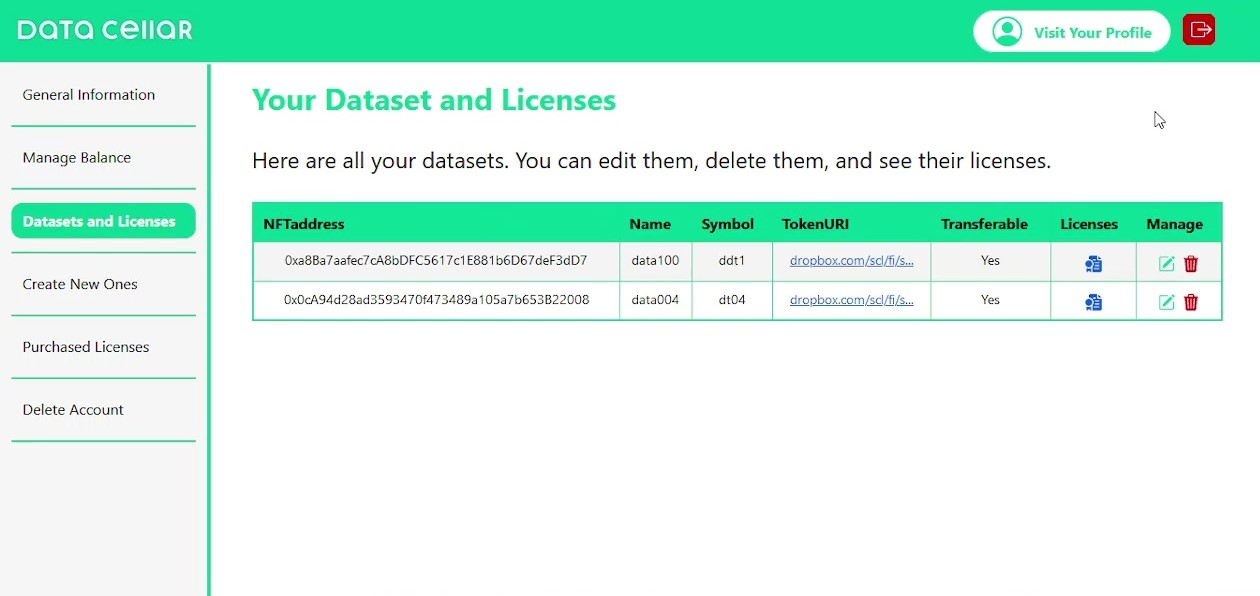
\includegraphics[width=0.8\textwidth]{Images/c6_8.jpg} 
    \caption{Page to view user's dataset and access their licenses.}
  \end{figure}

  \item \textbf{Create new Ones:} Here the user can create new datasets, i.e., add new datasets to the marketplace, or create new licenses related to an existing dataset 
  among its available ones. Datasets marked as transferable will be on the Home page of other users, allowing them to purchase their respective licenses.
  
  \begin{figure}[h]  
    \centering
    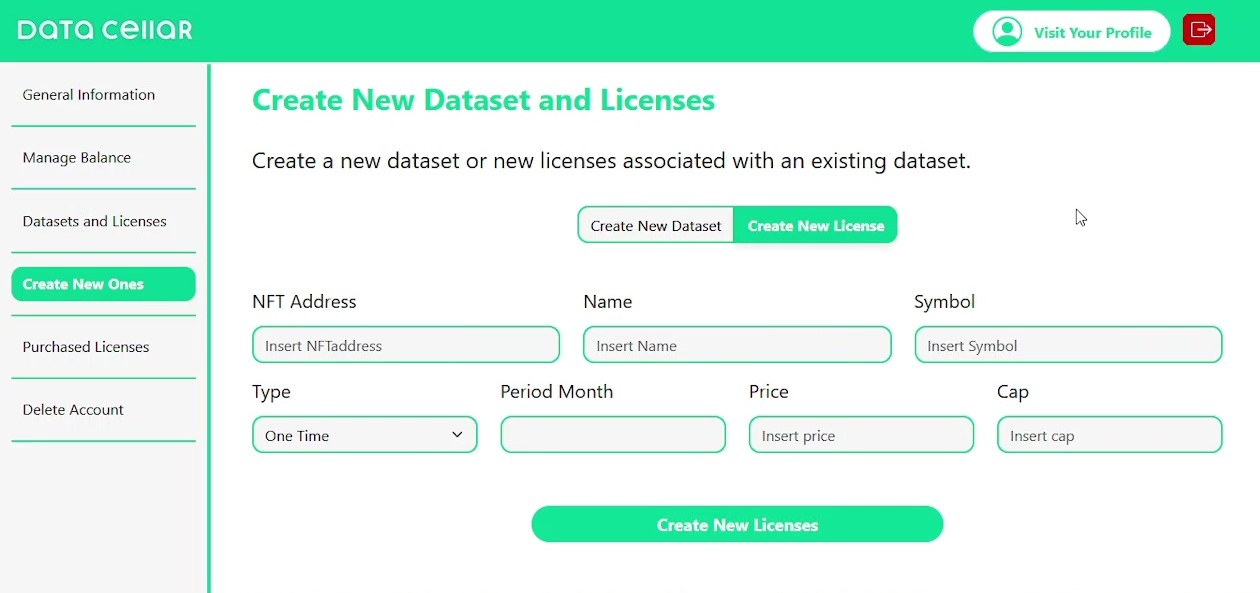
\includegraphics[width=0.8\textwidth]{Images/c6_9.jpg} 
    \caption{Page to create a new license or switch for new dataset. }
  \end{figure}
  
  \item \textbf{Purchased Licenses:} Shows the list of datasets for which the user has purchased at least one license. These licenses are visible by clicking on the 
  respective symbol leading to the dedicated page. Here the user can consume licenses, i.e., use them; periodic licenses can be used as many times as desired within the 
  validity period, while single-use licenses can be used a number of times equal to the amount of tokens available for it.
  
  \begin{figure}[h]  
    \centering
    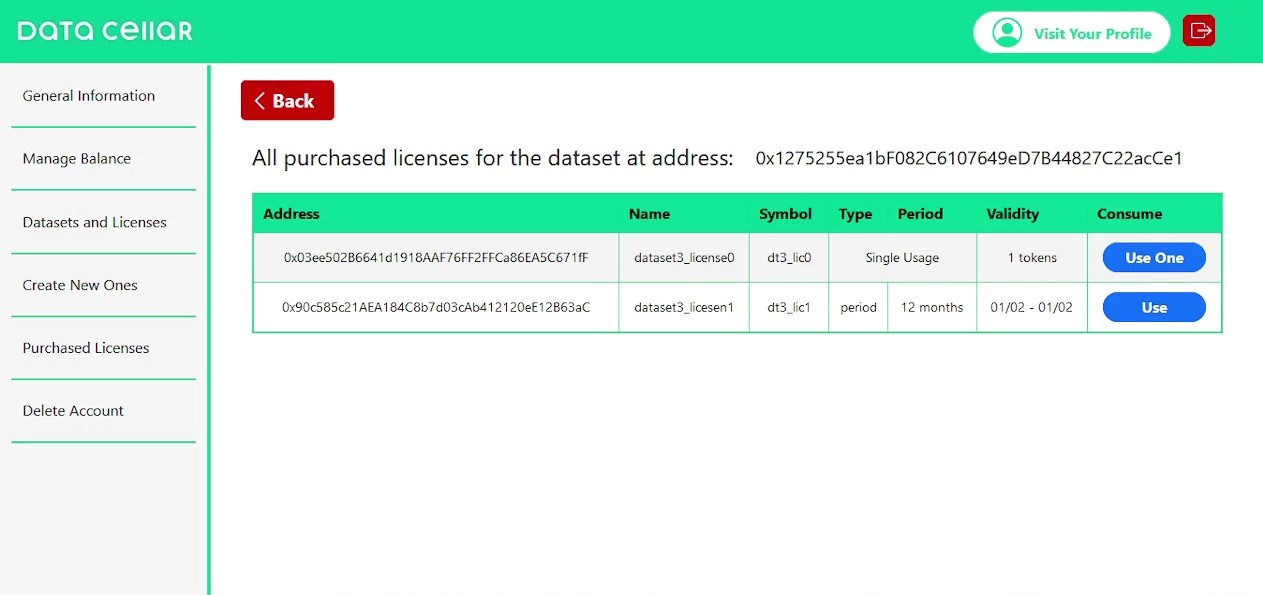
\includegraphics[width=0.8\textwidth]{Images/c6_10.jpg} 
    \caption{Page to view purchased licenses of specific dataset and use them.}
  \end{figure}
  
  \item \textbf{Delete Account:} This last page developed the latest smart contract function created for the \gls{ssi} management framework, which gives the user the ability to 
  delete their account, i.e., deregister. However, this function was not originally designed for this specific project, so it has limitations. In fact, by deleting an 
  account, the datasets, licenses and DataCellar tokens related to it and defined in the other smart contracts of the project are not deleted.

  \begin{figure}[h]  
    \centering
    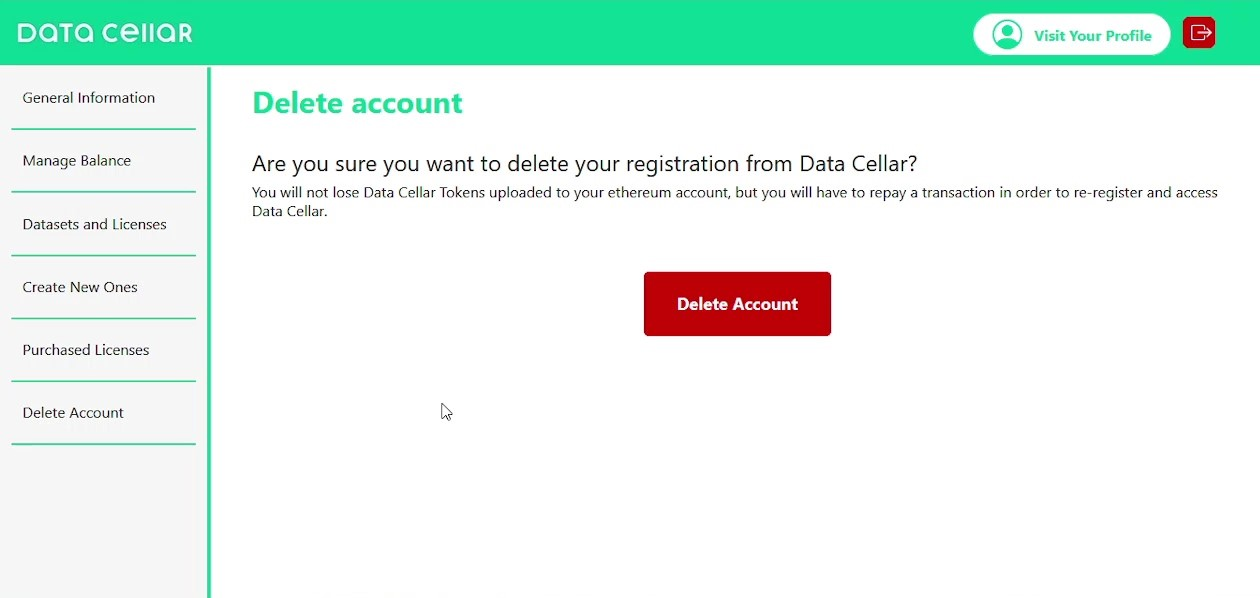
\includegraphics[width=0.8\textwidth]{Images/c6_11.jpg} 
    \caption{Page to delete user's account, performing de-registration.}
  \end{figure}

\end{itemize}